\chapter{Results and Analysis}
\label{ch:results}

\section{Evaluation Method}
\label{sec:eval-method}

All figures below were obtained from the running stack, not from
estimates. The system was started from a fresh clone with \code{make up}
and left running; four simulated days were reconciled by the Airflow DAG
without intervention. Metrics were read from the Prometheus endpoints and
the PostgreSQL bookkeeping tables (\code{batch\_runs},
\code{speed\_batch\_drift}, \code{dq\_issues},
\code{alert\_notifications}), which are the same sources the dashboards
and the daily report read. Where a figure could not be measured, it is
reported as not measured rather than estimated.

\section{The Consistency Argument}
\label{sec:consistency}

This section is the empirical justification for the entire architecture.

The speed layer applies a \textbf{10-simulated-minute watermark}; the
simulator injects lateness of up to \textbf{20 simulated minutes}. The
gap is deliberate. A watermark of 25 would catch everything, the two
layers would agree perfectly, and the project would have no evidence for
why the batch layer exists. A regression test fails if anyone raises it.
Figure~\ref{fig:consistency} shows the mechanism.

\begin{figure}[htbp]
\centering
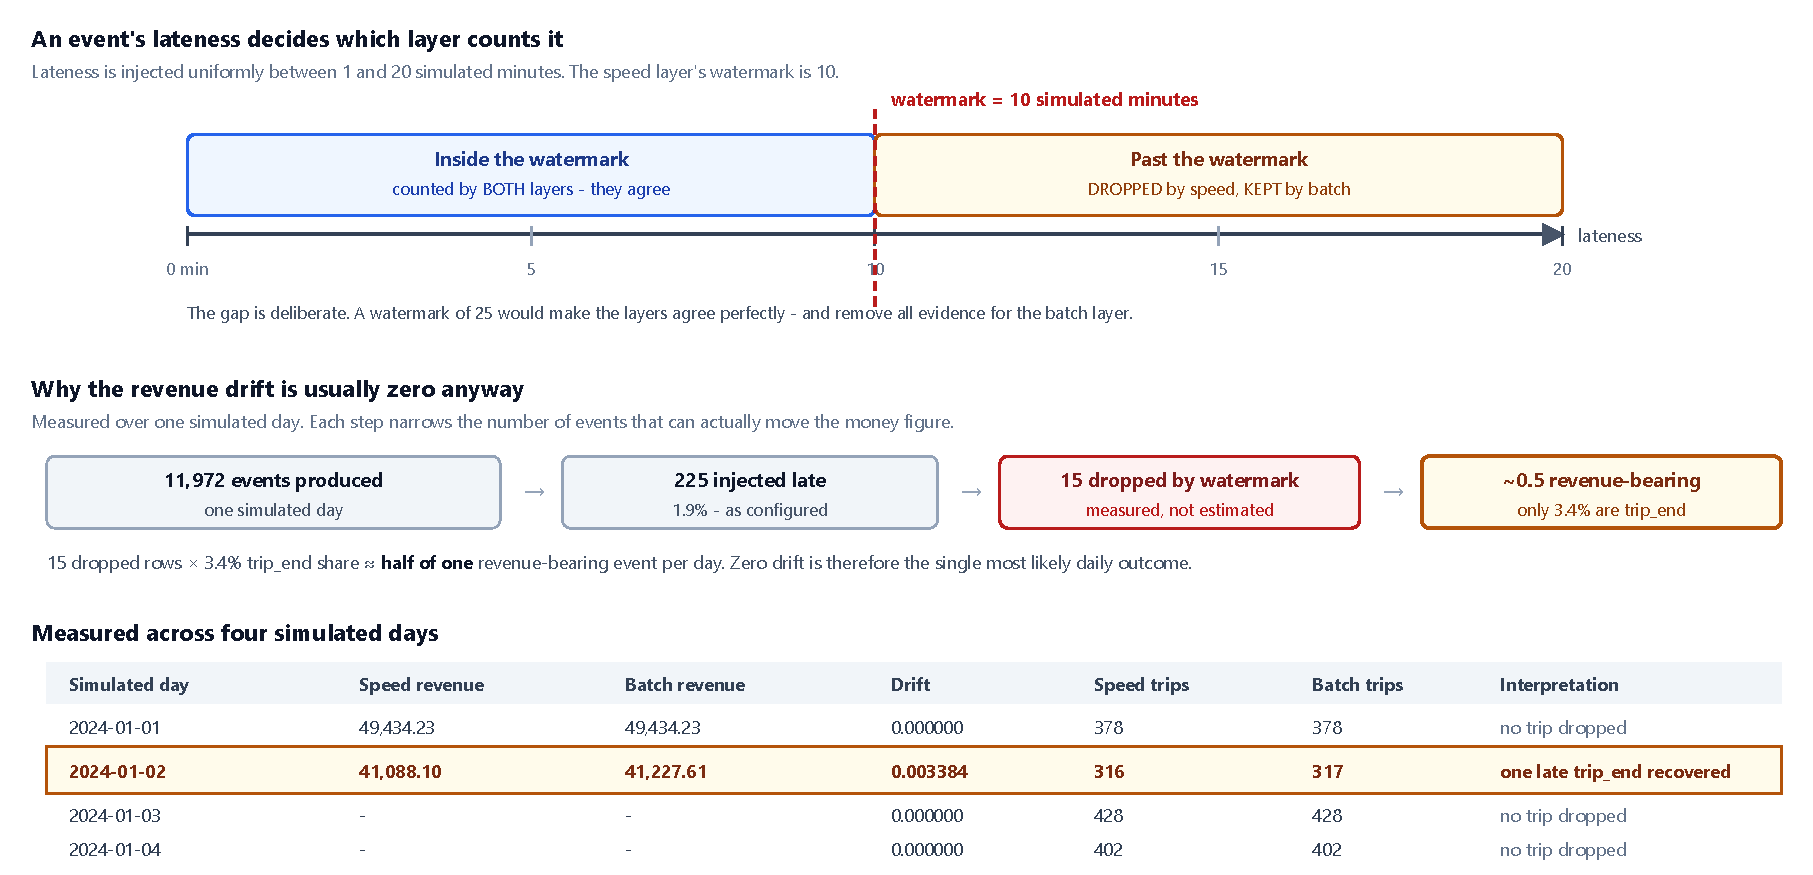
\includegraphics[width=\textwidth]{figures/fig2-consistency.pdf}
\caption[Why the two layers disagree]{Why the two layers disagree, and
by how much. An event's lateness decides which layer counts it; the
funnel shows why that translates into a near-zero revenue drift on a
typical day.}
\label{fig:consistency}
\end{figure}

\subsection{Results Over Four Simulated Days}

\begin{table}[htbp]
\centering
\caption{Reconciliation outcomes over four consecutive simulated days.
Revenue drift is the relative difference between the speed layer's and
the batch layer's daily revenue.}
\label{tab:four-days}
\begin{tabularx}{\textwidth}{@{}lRRRRR@{}}
\toprule
\textbf{Simulated day} & \textbf{Fleet margin} & \textbf{Unprof.} &
\textbf{Becoming unprof.} & \textbf{Dist. mismatch} &
\textbf{Revenue drift}\\
\midrule
2024-01-01 (partial) & 42.8\% & 6 & 0 & 2 & 0.000000\\
2024-01-02           & 38.3\% & 4 & 0 & \textbf{21} & \textbf{0.003384}\\
2024-01-03           & 45.8\% & 3 & 6 & 6 & 0.000000\\
2024-01-04           & 47.7\% & 4 & 7 & 4 & 0.000000\\
\bottomrule
\end{tabularx}
\end{table}

On \textbf{2024-01-02} the drift was 0.34\%, with
\code{speed\_trips}~=~316 against \code{batch\_trips}~=~317:
\textbf{exactly one late \code{trip\_end} event was dropped by the
watermark and recovered by the batch layer}. That single row is the
clearest evidence in the project --- the mechanism is real, measurable,
and attributable to a specific event.

\subsection{Why the Drift Is Usually Zero, and Why That Is the Stronger
Finding}
\label{sec:drift-zero}

We expected a visibly non-zero drift every day. Measuring why it is
usually zero produced a better argument than a dramatic number would
have.

\begin{table}[htbp]
\centering
\caption{The arithmetic of the watermark's loss, measured over one
simulated day.}
\label{tab:drift-arithmetic}
\begin{tabularx}{\textwidth}{@{}Xr@{}}
\toprule
\textbf{Quantity} & \textbf{Measured}\\
\midrule
Events produced (one day) & 11,972\\
Late events injected & 225 (1.9\%)\\
Rows dropped by the watermark & 15\\
Share of events that are \code{trip\_end} & 3.4\%\\
\textbf{Expected dropped revenue-bearing events} &
  $\mathbf{15 \times 0.034 \approx 0.5}$ \textbf{per day}\\
\bottomrule
\end{tabularx}
\end{table}

The watermark drops roughly \emph{half of one} revenue-bearing event per
day. Zero drift is therefore the single most likely outcome, and non-zero
appears on some days --- which is precisely what
Table~\ref{tab:four-days} shows.

\textbf{Two metrics, two jobs}, and this report uses both.
\code{fleet\_late\_rows\_dropped\_total} demonstrates the
\emph{mechanism} and is reliably non-zero;
\code{fleet\_speed\_batch\_drift\_ratio} demonstrates its \emph{financial
materiality} and is usually near zero. Reporting only the second would
understate the phenomenon; reporting only the first would overstate its
consequence.

The case for computing money in the batch layer was never ``the speed
layer is wildly wrong''. It is that \textbf{the speed layer's error is
unbounded in principle and unknowable in advance}. A watermark is a bet
on how late data arrives~\cite{akidau2015dataflow}; most days that bet is
won comfortably. But a partner resubmitting a corrected file for last
month is a restatement no watermark value addresses. Only recomputation
from an immutable archive does.

We deliberately did \emph{not} inflate the injected fault rates to
manufacture a larger figure. Reporting \code{0.000000} alongside the
arithmetic above is more defensible than reporting 8\% obtained by
quietly changing the simulator.

\section{Recomputation Demonstrated}
\label{sec:recompute}

Two experiments confirm the property the architecture exists to provide.

\textbf{Corrected resubmission.} Dropping a \code{v2} expense file for an
already-reconciled day made it pending again. The recompute produced
\textbf{the same 50 rows with different values} --- net profit
19,770.78 $\rightarrow$ 21,177.99 --- and the quarantined-row count fell
from~1 to~0. The load is delete-then-insert per date inside a single
transaction, so reruns are idempotent.

\textbf{Deterministic replay.} A manual trigger with
\code{\{"sim\_date": "2024-01-03", "force": true\}} recomputed that date
to \textbf{bit-identical figures} (net 24,902.95) with a fresh
\code{computed\_at} timestamp, confirming that recomputation from the
archive is deterministic, not merely repeatable.

Together these are the concrete form of the argument in
Section~\ref{sec:kappa-rejected}: the correction arrived on the file
channel, and the restatement was produced by re-reading one Parquet
partition, with no log replay involved at any point.

\section{Fault Handling and Data Quality}

The measured fault rates in Table~\ref{tab:faults} track the configured
rates closely, and every injected fault class was handled as designed:
malformed payloads were archived with bytes intact and dead-lettered by
the speed layer, schema-invalid events were rejected identically by both
layers' validation, and duplicates were removed by \code{event\_id} in
both the watermark window and the full-day batch dedup.

\section{Profitability Outcomes}

Across the four reconciled days the fleet margin ranged from 38.3\% to
47.7\%, with 3--6 of 50 vehicles flagged unprofitable on any given day.
The \code{becoming\_unprofitable} trend flag requires three reconciled
days before it will fire and correctly reported zero until that condition
was met on 2024-01-03.

The daily report is generated per simulated date and served at
\code{GET /reports/\{sim\_date\}}; a sample is included in the repository
at \code{docs/report-assets/}.

\section{Alerting Verification}
\label{sec:alerting-results}

Ten alert rules are defined. \textbf{Five have been verified firing
\emph{and delivered}} end to end through Alertmanager into the
\code{alert\_notifications} table: \code{TelemetryNotProduced},
\code{ExpenseFileLate}, \code{DLQRateHigh}, \code{BatchNotRunRecently}
and \code{ApiDown}. Delivery is demonstrable, not merely asserted.

A sixth, \code{BatchRunFailed}, fired but was \textbf{deliberately not
delivered}. A missing partner file causes the reconciliation to record a
failed run, so it fired alongside \code{ExpenseFileLate} for one root
cause. An Alertmanager inhibit rule suppresses it, confirmed in the API
with \code{inhibitedBy = 1}. Two alerts for one cause, where the second
is misleading --- nothing in the pipeline is broken, we are waiting on a
supplier --- is how alert channels become
ignored~\cite{beyer2016sre}.

Measured batch task durations were \code{compute\_vehicle\_day}
9.44\,s, \code{load\_batch\_views} 0.99\,s,
\code{reconcile\_profitability} 0.45\,s, and all others under 0.04\,s.

\section{Verification Summary}
\label{sec:verification}

\begin{table}[htbp]
\centering
\caption{Verification summary. Every row was run against the live stack.}
\label{tab:verification}
\begin{tabularx}{\textwidth}{@{}XX@{}}
\toprule
\textbf{Check} & \textbf{Result}\\
\midrule
Unit, PySpark and API tests & \textbf{202 passed}\\
End-to-end smoke test against the live stack & \textbf{28 / 28}\\
Fresh clone $\rightarrow$ single command &
  All 13 services healthy, pipeline serving live data\\
Simulated days reconciled & 4 clean days, 38--48\% fleet margin\\
Alert rules verified firing \emph{and delivered} &
  5 of 10 (a 6th fires but is intentionally inhibited)\\
Grafana panel queries returning live data & 23 of 23\\
\bottomrule
\end{tabularx}
\end{table}
